\documentclass{article}
\usepackage{pdflscape}
\usepackage[margin=1in]{geometry}
\usepackage{verbatim}
\usepackage{graphicx, float}
\usepackage{makecell}
\usepackage{amsmath}
\usepackage{amsfonts}
\usepackage{amssymb}
\usepackage{hyperref}
\usepackage{bookmark}
\usepackage{enumitem}


\author{Astrid Augusta Yu}
\title{CPE 233 Lab \#6 -- Complete ISA RISC-V MCU}
\date{\today}

\DeclareMathOperator\bit{bit}
\DeclareMathOperator\byte{byte}
\DeclareMathOperator\word{word}

\begin{document}
\maketitle

\tableofcontents

\section{Questions}

\begin{enumerate}    
    \item \textbf{Briefly describe how the AND gate in the RISC-V MCU schematic helps control the ability of the MCU to process interrupts.}

    The AND gate outputs MIE \& interrupt. Only when MIE is high can the interrupt be triggered. This is useful because it means an interrupt can only happen when the MCU isn't currently processing a previous interrupt. 

    \item \textbf{Based on the state diagram in Figure 14, would it be possible to assert the interrupt signal and not enter into an interrupt cycle? Briefly but completely explain. Assume the interrupt is unmasked.}

    Yes. If the interrupt is brought high during the LOAD state and low before the EXECUTE or WRITEBACK states, then it will not get detected. 
    
    \item \textbf{Interrupt architectures generally always automatically mask interrupts upon receiving an interrupt. Briefly but completely describe why this is a good approach, and a better approach than attempting to rely masking the interrupts under program control.}
    
    If the interrupt architecture didn't mask the interrupt, then a new interrupt may trigger while the last interrupt is still being processed. This can leave the RAM in an unpredictable state. Additionally, if the responsibility of masking goes to the program, then it would take longer to process any given interrupt. 
    
    \item \textbf{For the RISC-V MCU, there is only one state associated with the interrupt cycle, which means that it only requires one clock cycle to complete the interrupt cycle. Briefly but completely describe in general what dictates how many states (or clock cycles) a given MCU requires for the interrupt cycle. This question considers “states” and “clock cycles” as the same thing.}

    It is up to the CPU designer as to how many states the interrupt will need.
    
    \item \textbf{We generally consider interrupts “asynchronous” in nature. However, the RISC-V MCU is processes everything synchronously. Briefly describe what it means for the interrupts to be asynchronous and how exactly it is they are processed in an asynchronous manner.}

    The interrupts are asynchronous because they do not necessarily have to occur on the clock cycles. Technically, they are still processed on the clock signals, but they are detected and processed asynchronously from the normal flow of program instructions. 
    
    \item \textbf{Briefly but completely describe the major problem with the RISC-V MCU receiving an interrupt while it is in the act of processing an interrupt. For this problem, consider the interrupts as being masked when the MCU receives the interrupt.}

    If the interrupts are masked, then the MCU might miss an interrupt signal because it's too busy processing another interrupt. 
    
    \item \textbf{Briefly but completely describe the major problem with the RISC-V MCU receiving an interrupt while it is in the act of processing an interrupt. For this problem, consider the interrupts as being unmasked when the MCU receives the interrupt.}
    
    If the interrupts are unmasked, then the MCU may interrupt itself while processing another interrupt, which can potentially have unpredictable behavior.

    
\end{enumerate}

\pagebreak
\section{Programming Assignment}

\begin{verbatim}
# Test Code
	li x25, 0x65318945
    call sort
	li x25, 0x98558345
    call sort
	li x25, 0x87126354
    call sort
stop:
    j stop 

#---------------------------------------------------------------- 
#- Sorts the nibbles stored in a register using insertion sort.
#-
#- Parameters
#-      x25 - the nibbles to sort
#- Returns
#-      x25 - the sorted nibbles
#- Tweaked registers - x25
#----------------------------------------------------------------     
sort:
    addi sp, sp, -32
    sw x6, 0(sp)
    sw x7, 4(sp)
    sw x8, 8(sp)
    sw x9, 12(sp)
    sw x10, 16(sp)
    sw x11, 20(sp)
    sw x12, 24(sp)
    sw x13, 28(sp)

    andi x7, x25, 0xF   # x7 = output. Insert first element.
    srli x25, x25, 4    # Remove first element.
    li x12, 4           # Length of x7
    li x13, 32          # End at this value
    loop:
        beq x12, x13, end
        andi x9, x25, 0xF    # x9 = current unsorted element
        srli x25, x25, 4     # Move "read head" forwards
        li x10, 0            # Shift counter
        
        insertloop:    # Find the next element
            bge x10, x12, insertAtEnd   # if shift counter is at the end

            srl x6, x7, x10     # x6 = Shift sorted elements
            andi x8, x6, 0xF    # x8 = Current sorted element
            blt x8, x9, noinsert    # if sorted > unsorted
                slli x6, x6, 4      # Move everything > x8 1 nibble left
                or x6, x6, x9       # Place unsorted into this position
                sll x6, x6, x10     # Move back to actual position

                # Build mask for existing values
                li x11, -1
                sll x11, x11, x10 
                xori x11, x11, -1 # Toggle ALL bits
                and x7, x7, x11  # Mask existing values
                or x7, x7, x6    # Mask new values
                j endinsertloop
            noinsert:
                addi x10, x10, 4
                j insertloop

            insertAtEnd:         # Insert at the very end
                sll x9, x9, x12
                or x7, x7, x9
        endinsertloop:
            
        addi x12, x12, 4
        j loop
    end:
    mv x25, x7
    
    lw x6, 0(sp)
    lw x7, 4(sp)
    lw x8, 8(sp)
    lw x9, 12(sp)
    lw x10, 16(sp)
    lw x11, 20(sp)
    lw x12, 24(sp)
    lw x13, 28(sp)
    addi sp, sp, 32

    ret
\end{verbatim}

\pagebreak

\section{Hardware Design Assignment}

The RISC-V hardware will need to either support a new opcode or add a func3 code to an existing opcode. This is necessary in order for the MCU to be able to differentiate between the register + offset-based lw, lh, and lb. It will also need hardware to compute rs2 + rs1. This could be as minimal as simply using the ALU like it does for similar operations, but it could also be done by using a separate adder if necessary.

The assembler will need to be able to parse this instruction and determine the difference between this one and the existing lw, lh, and lb instructions. Additionally, it would need to emit the new opcode correctly.

The memory could be modified to support this new instruction by making it so that reading and writing is done simultaneously.

This could be useful for accessing an array at a variable location with a variable offset in a single instruction. Whereas before, in order to do this, the program would need to have a separate instruction for adding rs1 to rs2 prior to performing the array access, now, it only takes one instruction. 

\pagebreak

\section{HDL Models}
Note that these are somewhat-reformatted \texttt{git diff} outputs.

\subsection{CU\_DCDR}

\begin{verbatim}
@@ -39,11 +39,13 @@ module CU_DCDR(
     input br_eq, 
     input br_lt, 
     input br_ltu,
+    input int_taken,
+    
     input [6:0] opcode,   //-  ir[6:0]
     input [6:0] func7,    //-  ir[31:25]
     input [2:0] func3,    //-  ir[14:12] 
     output logic [3:0] alu_fun,
-    output logic [1:0] pcSource,
+    output logic [2:0] pcSource,
     output logic alu_srcA,
     output logic [1:0] alu_srcB, 
     output logic [1:0] rf_wr_sel
@@ -59,7 +61,8 @@ module CU_DCDR(
         LOAD   = 7'b0000011,
         STORE  = 7'b0100011,
         OP_IMM = 7'b0010011,
-        OP_RG3 = 7'b0110011
+        OP_RG3 = 7'b0110011,
+        OP_INT = 7'b1110011
     } opcode_t;
     opcode_t OPCODE; //- define variable of new opcode type
     
@@ -103,14 +106,16 @@ module CU_DCDR(
        
     always_comb begin 
         //- schedule all values to avoid latch
-        pcSource = 2'b00;  
-        rf_wr_sel = 2'b00; 
+        pcSource = 3'd0; // next
+        rf_wr_sel = 2'd0;  // pc_inc 
         
         alu_srcA = 1'b0;   
         alu_srcB = 2'b00;    
         alu_fun  = 4'b0000;
         
-        case(OPCODE)
+        if (int_taken) begin
+            pcSource = 3'd4;  // mtvec 
+        end else case(OPCODE)
             LUI: begin
                 alu_fun = 4'b1001;   // lui
                 alu_srcA = 1;        // u-imm 
@@ -126,12 +131,12 @@ module CU_DCDR(
             
             JAL: begin
                 rf_wr_sel = 2'd0;   // next pc
-                pcSource = 2'd3;     // jal
+                pcSource = 3'd3;     // jal
             end
             
             JALR: begin
                 rf_wr_sel = 2'd0;   // next pc
-                pcSource = 2'd1;       // jalr
+                pcSource = 3'd1;       // jalr
             end
             
             LOAD: begin
@@ -149,11 +154,11 @@ module CU_DCDR(
             
             BRANCH: 
                 pcSource = branch_cond   // Invert if invert bit 
-                    ? 2'd2      // Condition success, branch
-                    : 2'd0;     // Condition fail, next
+                    ? 3'd2      // Condition success, branch
+                    : 3'd0;     // Condition fail, next
             
             OP_IMM: begin
-                pcSource = 2'b00;  // next
+                pcSource = 3'd0;  // next
                 alu_srcA = 1'b0;   // rs1
                 alu_srcB = 2'd1;   // i imm
                 rf_wr_sel = 2'd3;  // alu result
@@ -161,15 +166,22 @@ module CU_DCDR(
             end
             
             OP_RG3: begin
-                pcSource = 2'b00;  // next
+                pcSource = 3'd0;  // next
                 alu_srcA = 0;   // rs1
                 alu_srcB = 2'd0;   // rs2
                 rf_wr_sel = 2'd3;  // alu result
                 alu_fun = op_alu_fun;  // translated func             
             end
+            
+            OP_INT: if (func3[0]) begin  // csrrw
+                rf_wr_sel = 2'd1;  // csr_reg
+                pcSource = 3'd0;  // next
+            end else begin  // mret
+                pcSource = 3'd5;  // mepc
+            end
 
             default: begin
-                 pcSource = 2'b00; 
+                 pcSource = 3'd0; 
                  alu_srcB = 2'b00; 
                  rf_wr_sel = 2'b00; 
                  alu_srcA = 1'b0; 
\end{verbatim}

\pagebreak

\subsection{CU\_FSM}

\begin{verbatim}
@@ -41,20 +41,24 @@ module CU_FSM(
     input intr,
     input clk,
     input RST,
+    input [2:0] func3,
     input [6:0] opcode,     // ir[6:0]
     output logic pcWrite,
     output logic regWrite,
     output logic memWE2,
     output logic memRDEN1,
     output logic memRDEN2,
-    output logic reset
+    output logic reset,
+    output logic csr_we,
+    output logic int_taken
   );
     
-    typedef enum logic [1:0] {
+    typedef enum logic [2:0] {
        st_INIT,
 	   st_FET,
        st_EX,
-       st_WB
+       st_WB,
+       st_INTR
     }  state_type; 
     state_type  NS,PS; 
       
@@ -68,12 +72,15 @@ module CU_FSM(
         LOAD   = 7'b0000011,
         STORE  = 7'b0100011,
         OP_IMM = 7'b0010011,
-        OP_RG3 = 7'b0110011
+        OP_RG3 = 7'b0110011,
+        OP_INT = 7'b1110011
     } opcode_t;
 	opcode_t OPCODE;    //- symbolic names for instruction opcodes
      
 	assign OPCODE = opcode_t'(opcode); //- Cast input as enum 
-	 
+	
+	state_type cmd_finish;
+	assign cmd_finish = intr ? st_INTR : st_FET;
 
 	//- state registers (PS)
 	always @(posedge clk) begin
@@ -91,6 +98,7 @@ module CU_FSM(
 		memWE2 = 1'b0;
         memRDEN1 = 1'b0;    
         memRDEN2 = 1'b0;
+        int_taken = 0;
                        
         case (PS)
             st_INIT: begin
@@ -115,48 +123,56 @@ module CU_FSM(
 					STORE: begin
                         regWrite = 0;
                         memWE2 = 1;
-                        NS = st_FET;
+                        NS = cmd_finish;
                     end
                     
 					BRANCH: begin
-                        NS = st_FET;
+                        NS = cmd_finish;
                     end
 					
 					LUI: begin
                         regWrite = 1;
-                        NS = st_FET;
+                        NS = cmd_finish;
                     end
                     
                     AUIPC: begin
                         regWrite = 1;
-                        NS = st_FET;
+                        NS = cmd_finish;
                     end
 					  
 					OP_IMM: begin 
                         regWrite = 1;	
                         memRDEN2 = 1;
-                        NS = st_FET;
+                        NS = cmd_finish;
                     end
 					
 					OP_RG3: begin 
                         regWrite = 1;	
                         memRDEN2 = 1;
-                        NS = st_FET;
+                        NS = cmd_finish;
                     end
 					
 	                JAL: begin
 					    regWrite = 1; 
-					    NS = st_FET;
+					    NS = cmd_finish;
                      end
                     
                     JALR: begin
 					    regWrite = 1; 
-					    NS = st_FET;
+					    NS = cmd_finish;
+                    end
+                    
+                    OP_INT: if (func3[0]) begin  // csrrw
+                        csr_we = 1;
+                        regWrite = 1;
+                        NS = cmd_finish;
+                    end else begin  // mret
+                        NS = st_FET;
                     end
 					 
                     default: begin 
                         regWrite = 0;
-                        NS = st_FET;
+                        NS = cmd_finish;
 					end
 					
                 endcase
@@ -166,10 +182,16 @@ module CU_FSM(
                 pcWrite = 0;
                 regWrite = 1; 
                 memRDEN2 = 1;
+                NS = cmd_finish;
+            end
+            
+            st_INTR: begin
+                pcWrite = 1;
+                int_taken = 1;
                 NS = st_FET;
             end
  
-            default: NS = st_FET;
+            default: NS = cmd_finish;
            
         endcase //- case statement for FSM states
     end
\end{verbatim}

\pagebreak

\subsection{OTTER\_MCU}
\begin{verbatim}
@@ -36,6 +36,7 @@ module OTTER_MCU #(
     logic [31:0] 
         pc, 
         pc_inc,
+        pc_next,
         ir, 
         reg_wd,
         rs1,
@@ -55,12 +56,18 @@ module OTTER_MCU #(
         i_type_imm, 
         j_type_imm,
         s_type_imm,
-        u_type_imm;
+        u_type_imm,
+        
+        mepc,
+        mtvec,
+        csr_reg;
     
     // Selectors
-    logic [1:0] pc_source, rf_wr_sel, alu_src_b;
-    logic [3:0] alu_fun;
+    logic [1:0] rf_wr_sel, alu_src_b;
+    logic [2:0] pc_source;
+
     logic alu_src_a;
+    logic [3:0] alu_fun;
     
     // Flags
     logic 
@@ -75,7 +82,11 @@ module OTTER_MCU #(
         
         br_eq,
         br_lt,
-        br_ltu;
+        br_ltu,
+        
+        int_taken,
+        csr_we,
+        csr_mie;
     
     assign iobus_addr = alu_result;
     assign iobus_out = rs2;
@@ -83,11 +94,11 @@ module OTTER_MCU #(
     // Multiplexers    
     always_comb case(rf_wr_sel)
         4'd0: reg_wd = pc + 4;
-        4'd1: reg_wd = 32'hdeadbeef;  // TODO change to CSR_reg
+        4'd1: reg_wd = csr_reg;
         4'd2: reg_wd = mem_dout;
         4'd3: reg_wd = alu_result;
     endcase
-    
+        
     assign alu_src_a_data = alu_src_a 
         ? u_type_imm 
         : rs1;
@@ -98,20 +109,52 @@ module OTTER_MCU #(
         4'd2: alu_src_b_data = s_type_imm;
         4'd3: alu_src_b_data = pc;
     endcase
+    
+    always_comb case(pc_source) 
+        3'd0: pc_next = pc_inc;
+        3'd1: pc_next = jalr;
+        3'd2: pc_next = branch;
+        3'd3: pc_next = jal;
+        3'd4: pc_next = mtvec;
+        3'd5: pc_next = mepc;
+        default: pc_next = 31'hdeadbeef;
+    endcase
+    
+    CSR csr(
+        .CLK(clk),
+        .RST(reset),
+        
+        .ADDR(ir[31:20]),
+
+        .INT_TAKEN(int_taken),
+        .WR_EN(csr_we),
+        .PC(pc),
+        .WD(rs1),
+        
+        .CSR_MIE(csr_mie),
+        .CSR_MEPC(mepc),
+        .CSR_MTVEC(mtvec),
+        .RD(csr_reg)
+    );
         
     // Submodules
     CU_FSM fsm(
         .clk(clk),
         
         .RST(RST), 
-        .intr(intr),
+        .intr(intr & csr_mie),
         .opcode(ir[6:0]),
-        
+        .func3(ir[14:12]),
+
         .pcWrite(pc_write),
         .regWrite(reg_write),
         .memWE2(mem_we2),
         .memRDEN1(mem_rden1),
         .memRDEN2(mem_rden2),
+        
+        .int_taken(int_taken),
+        .csr_we(csr_we),
+        
         .reset(reset)
     );
     
@@ -128,6 +171,7 @@ module OTTER_MCU #(
         .func7(ir[31:25]),
         .func3(ir[14:12]),
         
+        .int_taken(int_taken),
         .br_eq(br_eq),
         .br_lt(br_lt),
         .br_ltu(br_ltu),
@@ -142,12 +186,9 @@ module OTTER_MCU #(
     ProgramCounter prog_counter(
         .clk(clk),
 
-        .rst(reset),
-        .pc_source(pc_source),
         .pc_write(pc_write),
-        .jal(jal),
-        .jalr(jalr),
-        .branch(branch),
+        .rst(reset),
+        .next(pc_next),
         
         .addr(pc),
         .addr_inc(pc_inc)
\end{verbatim}

\begin{landscape}
    \section{Timing Diagram}

    \subsection*{Overview of the simulation}
    \includegraphics[width=\linewidth]{wf2a.png}

    Note that the analog waveform at the bottom is the PC's value duplicated to make it easier to see jumps and loops.

    Additionally, a different enum name was used for the opcode corresponding to the MRET and CSRRW instructions (OP\_INT instead of something like OP\_SYS). 

    \subsubsection*{Annotations}
    \begin{enumerate}[label=\Alph*.]
        \item First interrupt trigger.
        \item Second interrupt trigger.
        \item Third interrupt trigger, but MIE is low.
    \end{enumerate}

    \subsection*{Set mtvec}
    \includegraphics[width=\linewidth]{wf7.png}

    The OP\_INT at address 0x10 corresponds to the first CSRRW MTVEC.

    \subsection*{Enable interrupts}
    \includegraphics[width=\linewidth]{wf6.png}

    The OP\_INT at address 0x24 corresponds to the CSRRW MIE in the object dump. It brings MIE high.

    \subsection*{First Interrupt}
    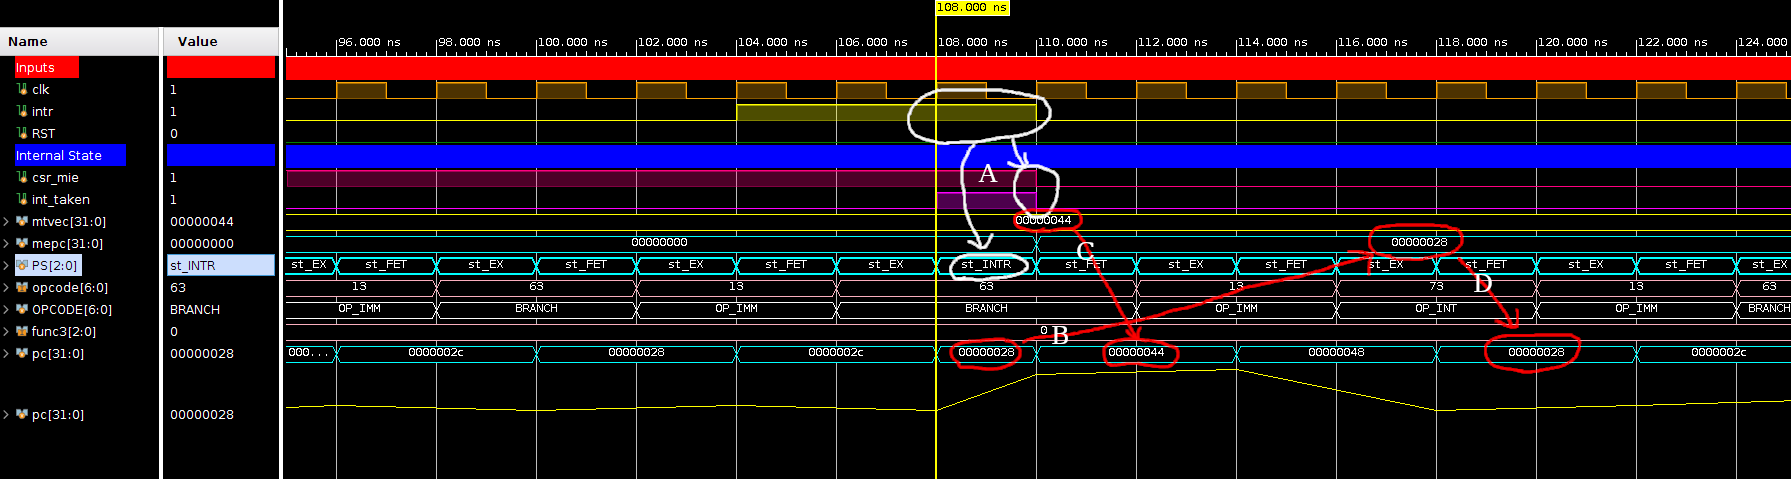
\includegraphics[width=\linewidth]{wf3.png}

    On the INTR cycle, the interrupt is detected. MIE is brought low and a jump occurs. 

    \begin{enumerate}[label=\Alph*.]
        \item The interrupt pulse causes the CU to enter the INTR state,int\_taken to be brought high and MIE to be brought low.
        \item mepc being set to original PC.
        \item The jump to mtvec.
        \item The mret call restores the original PC.
    \end{enumerate}

    \subsection*{CSRRW call 2}
    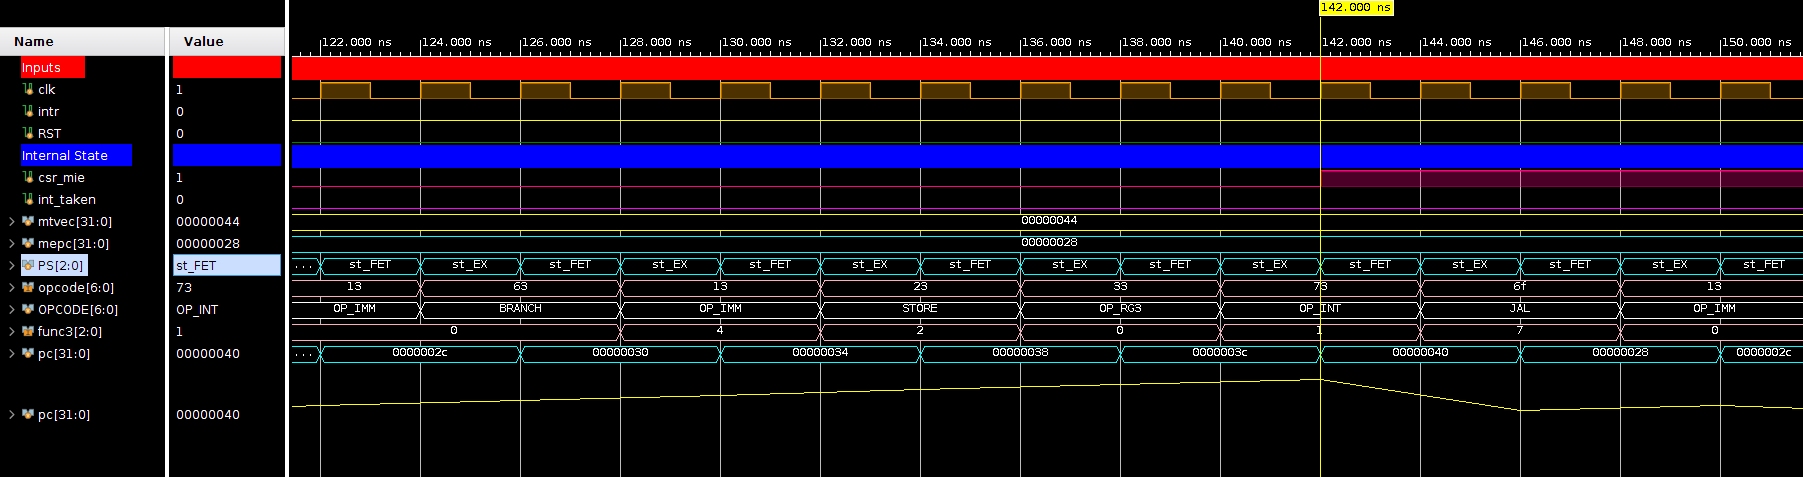
\includegraphics[width=\linewidth]{wf4.png}
    MIE is re-enabled.

    \subsection*{Second and Third Interrupts}
    \includegraphics[width=\linewidth]{wf5.png}
    \begin{enumerate}[label=\Alph*.]
        \item The interrupt pulse causes the CU to enter the INTR state,int\_taken to be brought high and MIE to be brought low.
        \item mepc being set to original PC.
        \item The jump to mtvec.
        \item The second interrupt pulse does not cause the interrupt state because MIE is low.
        \item The mret call restores the original PC.
    \end{enumerate}

\end{landscape}

\end{document}
